\documentclass[12pt]{article}
\usepackage[utf8]{inputenc}
\usepackage{graphicx} % Allows you to insert figures
\usepackage{amsmath} % Allows you to do equations
\usepackage{fancyhdr} % Formats the header
\usepackage{geometry} % Formats the paper size, orientation, and margins
\usepackage[style=authoryear-ibid,backend=biber]{biblatex} % Allows you to do citations - does Harvard style and compatible with Zotero

% PARA IMAGNES E SUBIMAGENS
\usepackage{graphicx}
\usepackage{subcaption}
\usepackage{mwe}

\usepackage[section]{placeins}
\usepackage{hyperref}
\usepackage{listings}

\usepackage{amsmath}

\addbibresource{Example.bib} % Tells LaTeX where the citations are coming from. This is imported from Zotero
\usepackage[english]{babel}
\usepackage{csquotes}
\renewcommand*{\nameyeardelim}{\addcomma\space} % Adds comma in in-text citations
\linespread{1.25} % About 1.5 spacing in Word
\setlength{\parindent}{0pt} % No paragraph indents
\setlength{\parskip}{1em} % Paragraphs separated by one line
\renewcommand{\headrulewidth}{0pt} % Removes line in header
\geometry{legalpaper, portrait, margin=1in}
\setlength{\headheight}{14.49998pt}

\begin{document}
\begin{titlepage}
   \begin{center}
        \vspace*{5cm}

        \Huge{Lesson 3 - Texture and Interaction}

        \vspace{0.5cm}
        \LARGE{} % Optional Subtitle Below
            
        \vspace{3 cm}
        \Large{Course: Information Visualization - 44156}
       
        \vspace{0.25cm}
        \large{André Fernandes (97977) 50.0\%, Gonçalo Machado (98359) 50.0\%}
       
        \vspace{3 cm}
        \Large{27/12/2023}
        
        \vspace{0.25 cm}
        \Large{Class - TP2}
        
        \vspace{5cm}
        \Large{Developed \emph{software} can be found \textbf{\href{https://github.com/goncalo-machado/VI}{here}}.}
       

       \vfill
    \end{center}
\end{titlepage}

\setcounter{page}{2}
\pagestyle{fancy}
\fancyhf{}
\rhead{\thepage}
\lhead{Lesson 3 - Texture and Interaction - André and Gonçalo - VI}

% -> Para fazer citações usamos: \autocite{}
%%%%%%%%%%%%%%%%%%%%%%%%%%%%%%%%%%%%%%%%%%%%%%%%%%%%%%%%%%
\section*{Introduction}
\label{intro}

In the Lesson 3 of the Computer Graphics module, the focus will be on textures and interactions. Here, we'll understand what are textures, how to apply them to models and how they interact with light. We will also use some interaction to change the scene and the models within, while creating a representation of the earth and moon, their interaction with each other and their interaction in a light that simulates the sun.

%%%%%%%%%%%%%%%%%%%%%%%%%%%%%%%%%%%%%%%%%%%%%%%%%%%%%%%%%%
\section*{3.1 - Using a texture in a plane}
\label{sec:ex_31}

For the first exercise we got to use as a base, once again, the rotating cube but now, as a material, we've used a material's map attribute to apply the Lena.jpg image as the plane texture. To read the image we have used given code.\newline
Before all of this, we should have change the cube to a plane geometry.\newline
In Figure \ref{fig:ex_31} are represented 3 different results were the size of the plane was changed, the THREE.PlaneGeometry parameters.

\begin{figure}[!h]
\centering
    \begin{subfigure}{.33\textwidth}
        \centering
        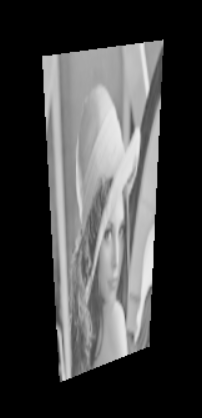
\includegraphics[width = \textwidth]{figs/ex_31_1.png}
        \caption{THREE.PlaneGeometry parameters (1, 3)}
        \label{fig:ex_31_1}
    \end{subfigure}%
    \begin{subfigure}{.33\textwidth}
        \centering
        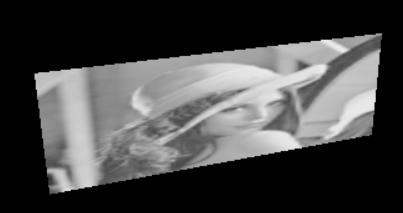
\includegraphics[width = \textwidth]{figs/ex_31_2.png}
        \caption{THREE.PlaneGeometry parameters (3, 1)}
        \label{fig:ex_31_2}
    \end{subfigure}
    \begin{subfigure}{.33\textwidth}
        \centering
        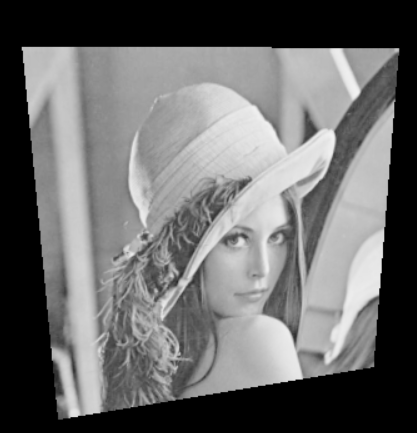
\includegraphics[width = \textwidth]{figs/ex_31_3.png}
        \caption{THREE.PlaneGeometry parameters (3, 3)}
        \label{fig:ex_31_3}
    \end{subfigure}
\caption{Results of 3.1 - Using a texture in a plane}
\label{fig:ex_31}
\end{figure}

\noindent
As it possible to see, in Figure \ref{fig:ex_31_1} we've used as parameters (1, 3) and the image got stretched vertically; in Figure \ref{fig:ex_31_2} the parameters were (3, 1) and now, the image got stretched horizontally; finally, using (3, 3) as parameters, in Figure \ref{fig:ex_31_3}, the image is represented without distortion, since the original image is a square.\par

NOTE: the angle of the plane is because of an animation that is rotating the plane.


%%%%%%%%%%%%%%%%%%%%%%%%%%%%%%%%%%%%%%%%%%%%%%%%%%%%%%%%%%
\section*{3.2 - Texture on a cube}
\label{ex_32}

In this exercise, which is based on the previous, we were asked to change the geometry back to a cube and see how the image was mapped.

\begin{figure}[!h]
    \centering
        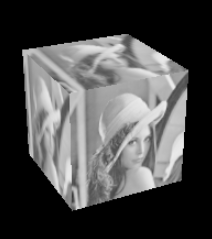
\includegraphics[width = 0.7\textwidth]{figs/ex_32_lena.png}
        \caption{Mapping  lena.png to texture of cube}
        \label{figs:ex_32_lena}
\end{figure}

As we can see in Figure \ref{figs:ex_32_lena}, the image was mapped to all six faces of the cube.

After, we were asked to map different images for each face of the cube as texture.\par

To achieve that, it is necessary to aggregate all the textures in a materials variable using the push command:
\begin{lstlisting}

const materials = [];
for (var i = 1; i <= 6; i++){
    materials.push(new THREE.MeshBasicMaterial({ map: new
                    THREE.TextureLoader().load('images/Im'+i+'.jpg') }));
}

\end{lstlisting}

The results are represented in Figure \ref{fig:ex_32}.

\begin{figure}[!h]
\centering
    \begin{subfigure}{.5\textwidth}
        \centering
        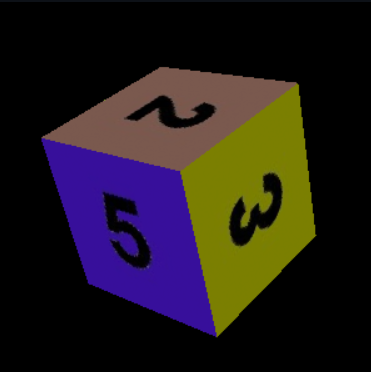
\includegraphics[width = \textwidth]{figs/ex_32_1.png}
        \caption{Expected result.}
        \label{fig:ex_32_1}
    \end{subfigure}%
    \begin{subfigure}{.5\textwidth}
        \centering
        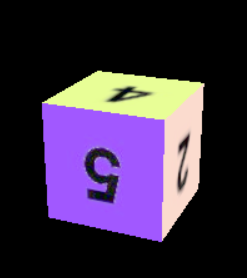
\includegraphics[width = \textwidth]{figs/ex_32_2.png}
        \caption{Result gotten.}
        \label{fig:ex_32_2}
    \end{subfigure}
\caption{Results of 3.2 - Texture on a cube}
\label{fig:ex_32}
\end{figure}

%%%%%%%%%%%%%%%%%%%%%%%%%%%%%%%%%%%%%%%%%%%%%%%%%%%%%%%%%%
\section*{3.3 - Texture and Lighting}
\label{ex_33}

Different from the first two exercises, this one asks for a creation of a new program with the goal of visualizing a sphere of radius 1 using 32 segments in width and height.\par

After the sphere creation, consulting the work done in Lesson 2, the next step was apply the earth\_surface\_2048.jpg as texture to the sphere. For that, the strategy followed was the same as the Exercise 3.1.\par

Then, we were told to change the material type to MeshPhongMaterial. This material type requires light so, the next step was adding an ambient light with the value 0x333333 and a directional light with direction (1,0,0) and with the value 0xfffff representing the sun, following the steps used in Lesson 2.

\begin{figure}[!h]
    \centering
        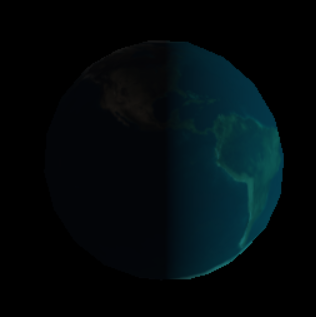
\includegraphics[width = 0.7\textwidth]{figs/ex_33.png}
        \caption{Results of 3.3 - Texture and Lighting}
        \label{figs:ex_33}
\end{figure}

Besides the result obtain in Figure \ref{figs:ex_33}, we had to implement an animation. This animation consists on a rotation around the y axis of 0.0025 rad and, before that, a fixed rotation on the Z axis of 0.41 rad.
\begin{lstlisting}

sphere.rotation.y += 0.0025;
sphere.rotation.z = 0.41;

\end{lstlisting}

\noindent
Note that the rotation parameter in the Z axis only as an = instead of += because this is a single rotation, that is, is fixed and don't change over time like the Y axis one, that represents the Earth rotation.

%%%%%%%%%%%%%%%%%%%%%%%%%%%%%%%%%%%%%%%%%%%%%%%%%%%%%%%%%%
\section*{3.4 - Interaction}
\label{ex_34}

In this exercise, the only task was to add an event that responded to a keydown (pressing a keyboard key) event, that is, adding the possibility to our program know that we were pressing keys and giving it the possibility to read them/know what key were we pressing.\par

For that, we just implemented in the code before the following given code:
\begin{lstlisting}

document.addEventListener("keydown", onDocumentKeyDown, false);

function onDocumentKeyDown(event){ 
    // Get the key code of the pressed key 
    var keyCode = event.which;
    console.log("Key  " + keyCode);
}

\end{lstlisting}

%%%%%%%%%%%%%%%%%%%%%%%%%%%%%%%%%%%%%%%%%%%%%%%%%%%%%%%%%%
\section*{3.5 - Lighting activation}
\label{ex_35}

Now, with the possibility to interact with our program by pressing keyboard keys, we were asked to modify the previews code so that there was the possibility to turn on/off the directional light via the L key or the possibility to turn the material of the sphere from MeshPhongMaterial back to MeshBasicMaterial and vice-versa. We chose to make both options possible, with the option of turning the directional light on/off via the L key and the option of turning the material of the sphere to MeshPhongMaterial/MeshBasicMaterial via the K key.\par

To do this, in the function onDocumentKeyDown, we created a switch case using the keyCode as the expression, and with the following cases:
\begin{lstlisting}

case 76:
    if (light_on){
        scene.remove(directionalLight);
        light_on = false;
        console.log('Directional Light Off');
    }else{
        scene.add(directionalLight);
        light_on = true;
        console.log('Directional Light On');
    }
    break;
// k key
case 75:
    if (phong_mesh){
        sphere.material = basic_material;
        phong_mesh = false;
        console.log('Using Basic Material');
    }else{
        sphere.material = phong_material;
        phong_mesh = true;
        console.log('Using Phong Material');
    }
    break;

\end{lstlisting}

\noindent

\begin{figure}[!h]
\centering
    \begin{subfigure}{.5\textwidth}
        \centering
        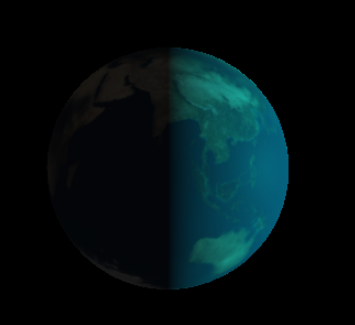
\includegraphics[width = \textwidth]{figs/ex_35_normal.png}
        \caption{Starting Model}
        \label{fig:ex_35_normal}
    \end{subfigure}%
    \begin{subfigure}{.5\textwidth}
        \centering
        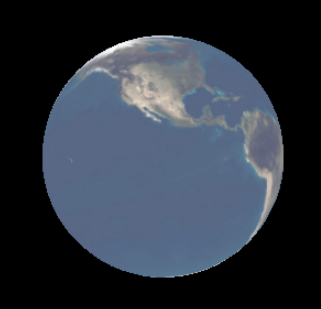
\includegraphics[width = \textwidth]{figs/ex_35_material.png}
        \caption{Basic Material Used}
        \label{fig:ex_35_material}
    \end{subfigure}
    \begin{subfigure}{.5\textwidth}
        \centering
        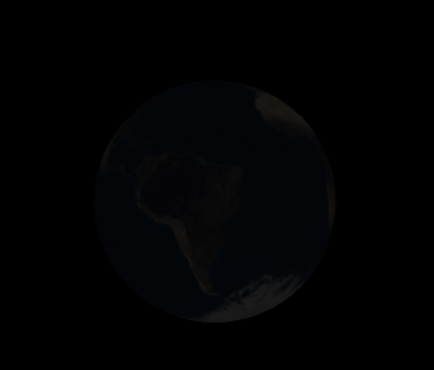
\includegraphics[width = \textwidth]{figs/ex_35_light.png}
        \caption{Directional Light Off}
        \label{fig:ex_35_light}
    \end{subfigure}
\caption{Different methods used}
\label{fig:ex_35}
\end{figure}

As we can see in Figure \ref{fig:ex_35_material}, when using a MeshBasicMaterial, the sphere does not interact with light, so we see the original image used. On Figure \ref{fig:ex_35_light}, we can see that with the directional light turned off, the sphere is barely visible, and does not become invisible due to the ambient light.

It was also requested the possibility to increase/decrease the light intensity using the + and - keys. For that, the logic was the same:
\begin{lstlisting}

// + key
case 107:
    directionalLight.intensity += 0.1;
    console.log('Increased directional light intensity to ' + directionalLight.intensity.toFixed(1));
    break;
// - key
case 109:
    if (directionalLight.intensity >= 0){
        directionalLight.intensity -= 0.1;
        console.log('Reduced directional light intensity to ' + directionalLight.intensity.toFixed(1));
    }else{
        console.log('Directional light intensity cannot be reduced further');
    }
    break;

\end{lstlisting}

\noindent
Now, instead of adding/removing something from the scene, we just incremented the intensity parameter of the light. We also checked if the intensity was bigger than 0 before decreasing the intensity, since a negative intensity makes no sense and is no different than a intensity with value 0.

To note that the ASCII code for the 'L' key is 76, for the 'K' key is 75, for the '+' key is 107 and for the '-' key is 109. 

%%%%%%%%%%%%%%%%%%%%%%%%%%%%%%%%%%%%%%%%%%%%%%%%%%%%%%%%%%
\section*{3.6 - Modify position and rotation}
\label{ex_36}

In the exercise 3.6, the goal was the same as the previews exercise, related to interaction.\par

This time, when the arrow keys were pressed, left and right, the rotation speed around the yy axis would increase/decrease and, the when up/down keys were pressed, the inclination of the model around the zz axis would change.\par

Once again, we added new cases on the function of Exercise 3.4:
\begin{lstlisting}

// left arrow key
case 37:
    rotation_speed -= 0.0005;
    console.log('Increased rotation speed to ' + rotation_speed.toFixed(4));
    break;
// right arrow key
case 39:
    rotation_speed += 0.0005;
    console.log('Increased rotation speed to ' + rotation_speed.toFixed(4));
    break;
// up arrow key
case 38:
    sphere.rotation.z += 0.01;
    console.log('Increased sphere inclination to ' + sphere.rotation.z.toFixed(2));
    break;
// down arrow key
case 40:
    sphere.rotation.z -= 0.01;
    console.log('Increased sphere inclination to ' + sphere.rotation.z.toFixed(2));
    break;

\end{lstlisting}

\noindent

The code was also changed to use the rotation\_speed variable in the animation function.

\noindent
So, when the user pressed the arrow keys, he could interact with rotation parameters of the sphere.

%%%%%%%%%%%%%%%%%%%%%%%%%%%%%%%%%%%%%%%%%%%%%%%%%%%%%%%%%%
\section*{3.7 - Concatenation of transformations / addition of the Moon}
\label{ex_37}

For the finally exercise, we had to add a new model, the Moon, with the same logic of the Earth, adding a new sphere with a specifc texture, the moon\_1024.jpg. Its parameters are the following:
\begin{lstlisting}

DISTANCE_FROM_EARTH = 356400;
PERIOD = 28;
INCLINATION = 0.089;
SIZE_IN_EARTHS = 1 / 3.7;
EARTH_RADIUS = 6371;

\end{lstlisting}

As it occurs in real life, the Moon rotates around the Earth and around itself. To get the rotation around the Earth we need to create the Moon as a child of the Earth so that the moon gets influenced by the Earth's transformations. This is an automatic process because the transformation matrices of the two objects are multiplied.\newline
To initialize the Moon in its correct position we added the following code lines:
\begin{lstlisting}

var distance = DISTANCE_FROM_EARTH / EARTH_RADIUS;
moon.position.set(Math.sqrt(distance / 2), 0,-Math.sqrt(distance / 2));


\end{lstlisting}

\noindent
Then, its animation is obtained by the following:

\begin{lstlisting}

// Rotate the moon so it shows its moon-face toward earth
moon.rotation.y = Math.PI;
moon.rotation.x = INCLINATION;
// For animation 
moon.rotation.y += (earth.rotation.y / PERIOD);

\end{lstlisting}

The result obtained are illustrated in three different angles, in Figure \ref{fig:ex_37}, so it is possible to have a representation of the Moon's movement, its rotation, around the Earth.

\begin{figure}[!h]
\centering
    \begin{subfigure}{.33\textwidth}
        \centering
        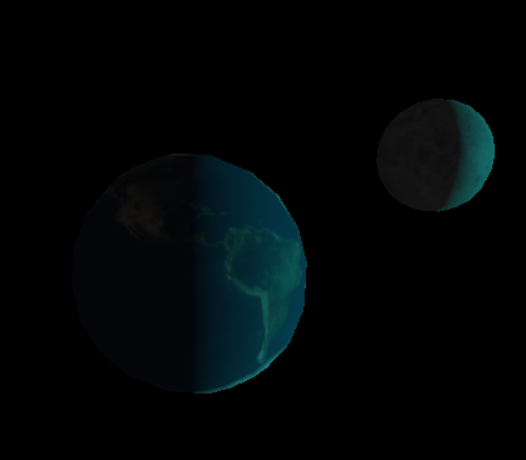
\includegraphics[width = \textwidth]{figs/ex_37_1.png}
        \caption{One angle.}
        \label{fig:ex_37_1}
    \end{subfigure}
    \begin{subfigure}{.33\textwidth}
        \centering
        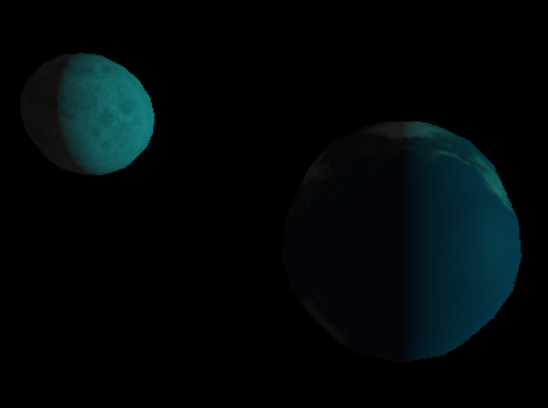
\includegraphics[width = \textwidth]{figs/ex_37_2.png}
        \caption{Different angle.}
        \label{fig:ex_37_2}
    \end{subfigure}
    \begin{subfigure}{.33\textwidth}
        \centering
        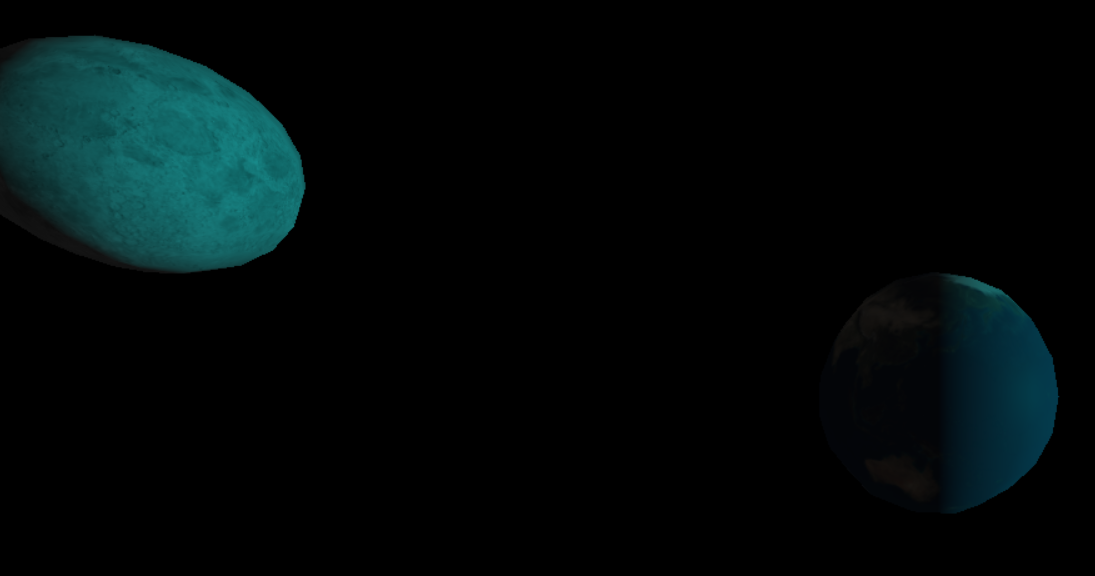
\includegraphics[width = \textwidth]{figs/ex_37_3.png}
        \caption{Another angle.}
        \label{fig:ex_37_3}
    \end{subfigure}
\caption{Results of 3.7 - Concatenation of transformations / addition of the Moon}
\label{fig:ex_37}
\end{figure}

As an addiction to the exercise, we added a new interaction that allow the user change the texture applied on the sphere object that represents the Earth.\par

For that, it was necessary to add a new condition to the that when 'C' key is pressed, a function is called and the texture change is performed:

\begin{lstlisting}

var texloader = new THREE.TextureLoader();
var earth_tex = texloader.load("../images/earth_surface_2048.jpg");
const earth_textures = [
    "../images/earth_surface_2048.jpg",
    "../images/earth_clouds_1024.png",
    "../images/earth_normal_2048.jpg",
    "../images/earth_specular_2048.jpg",
    "../images/earth_atmos_2048.jpg",
  ];

...

function onDocumentKeyDown(event){ 

    ...

    case 67:
    // Increment the texture index (loop back to the start if needed)
    current_texture_index = (current_texture_index + 1) % earth_textures.length;
    
    const next_texture_path = earth_textures[current_texture_index];
    const next_texture = texloader.load(next_texture_path);
    console.log("Earth Texture: " + next_texture_path);
    
    // Update both materials map with the new texture
    basic_material.map = next_texture;
    phong_material.map = next_texture;

    basic_material.needsUpdate = true;
    phong_material.needsUpdate = true;

    break;

}

\end{lstlisting}

\noindent
The first step is increment the variable that is the image index and, if this value is equal to the number of images available minus 1 (because index starts in 0), the operation returns a 0 and the variable is reset, that is, it is attributed the 0 value. After, we get the image path from the earth\_textures list using an variable as index. Then, we set both materials map as the texture, and we update the materials.\newline
All texture can be checked in Figure \ref{fig:ex_37_extra}.

\begin{figure}[!h]
\centering
    \begin{subfigure}{.4\textwidth}
        \centering
        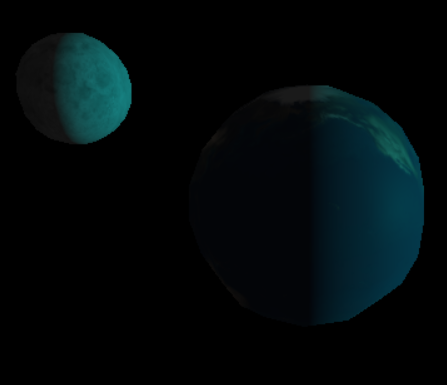
\includegraphics[width = \textwidth]{figs/ex_37_1_extra.png}
        \caption{1st Texture: earth\_atmos\_2048.}
        \label{fig:ex_37_1_extra}
    \end{subfigure}
    \begin{subfigure}{.4\textwidth}
        \centering
        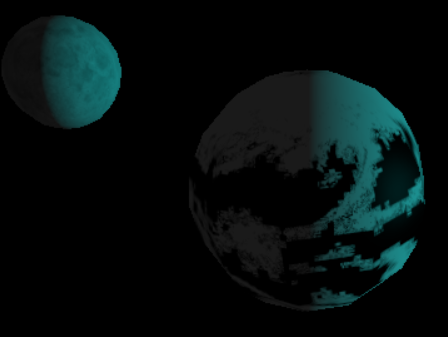
\includegraphics[width = \textwidth]{figs/ex_37_2_extra.png}
        \caption{2nd Texture: earth\_clouds\_1024.}
        \label{fig:ex_37_2_extra}
    \end{subfigure}
    \begin{subfigure}{.4\textwidth}
        \centering
        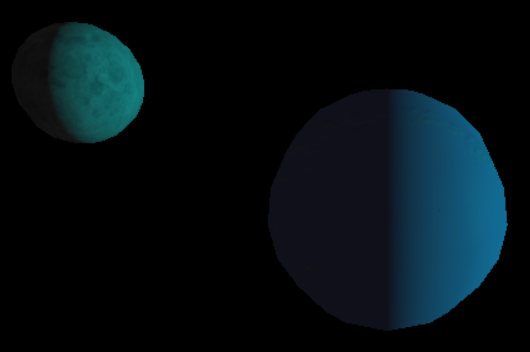
\includegraphics[width = \textwidth]{figs/ex_37_3_extra.png}
        \caption{3rd Texture: earth\_normal\_2048.}
        \label{fig:ex_37_3_extra}
    \end{subfigure}
    \begin{subfigure}{.4\textwidth}
        \centering
        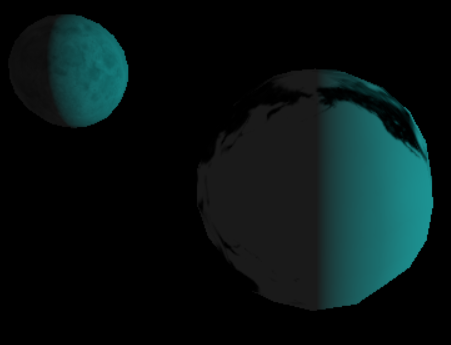
\includegraphics[width = \textwidth]{figs/ex_37_4_extra.png}
        \caption{4th Texture: earth\_specular\_2048.}
        \label{fig:ex_37_4_extra}
    \end{subfigure}
    \begin{subfigure}{.4\textwidth}
        \centering
        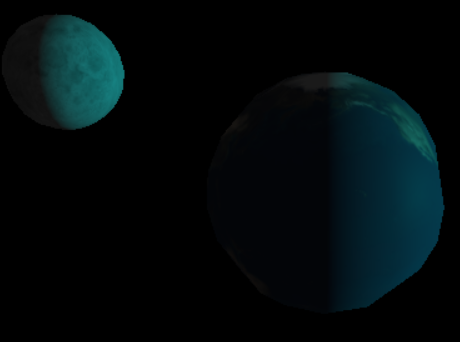
\includegraphics[width = \textwidth]{figs/ex_37_5_extra.png}
        \caption{5th Texture: earth\_surface\_2048.}
        \label{fig:ex_37_5_extra}
    \end{subfigure}
\caption{Results of 3.7 - Extra Work.}
\label{fig:ex_37_extra}
\end{figure}

%%%%%%%%%%%%%%%%%%%%%%%%%%%%%%%%%%%%%%%%%%%%%%%%%%%%%%%%%%
\section*{Conclusion}
\label{Concl}

To sum up the Lesson 3 - Texture and Interaction, covering textures, lighting, and interactive elements, the exercises explored applying textures to different geometries, incorporating lighting and introducing user interaction through keyboard input. Overall, the lesson provided a hands-on experience in creating visually compelling and interactive 3D scenes by combining textures, lighting, and user-driven transformations.\par

Finally, it is possible to say that the exercises were completed with success as the results were as expected.

%%%%%%%%%%%%%%%%%%%%%%%%%%%%%%%%%%%%%%%%%%%%%%%%%%%%%%%%%%

\end{document}

